%---------------------------------------------------------------------
%
%                          Cap�tulo 5
%
%---------------------------------------------------------------------
%
% 05Bibliografia.tex
% Copyright 2009 Marco Antonio Gomez-Martin, Pedro Pablo Gomez-Martin
%
% This file belongs to the TeXiS manual, a LaTeX template for writting
% Thesis and other documents. The complete last TeXiS package can
% be obtained from http://gaia.fdi.ucm.es/projects/texis/
%
% Although the TeXiS template itself is distributed under the 
% conditions of the LaTeX Project Public License
% (http://www.latex-project.org/lppl.txt), the manual content
% uses the CC-BY-SA license that stays that you are free:
%
%    - to share & to copy, distribute and transmit the work
%    - to remix and to adapt the work
%
% under the following conditions:
%
%    - Attribution: you must attribute the work in the manner
%      specified by the author or licensor (but not in any way that
%      suggests that they endorse you or your use of the work).
%    - Share Alike: if you alter, transform, or build upon this
%      work, you may distribute the resulting work only under the
%      same, similar or a compatible license.
%
% The complete license is available in
% http://creativecommons.org/licenses/by-sa/3.0/legalcode
%
%---------------------------------------------------------------------

\chapter{Pruebas con usuarios}
\label{cap5}
\label{cap:pruebas}

En el cap\'itulo anterior hemos visto c\'omo se ha realizado la implementaci\'on de las diferentes caracter\'isticas de la aplicaci\'on de Android y Unity. Adem\'as de esto, se han explicado cada una de las clases que contiene la librer\'ia y de las que deber\'a hacer uso el desarrollador.\\
En este cap\'itulo se van a realizar pruebas de rendimiento de la herramienta con usuarios. Para que estas pruebas puedan realizarse, se ha introducido la librer\'ia en un proyecto terminado. Estas pruebas se realizar\'an con usuarios ajenos al proyecto y los resultados marcaran los aspectos a mejorar en futuras revisiones de este trabajo. \\

%-------------------------------------------------------------------
\section{Integraci\'on de la librer\'ia en juegos finalizados}
%-------------------------------------------------------------------

Unity ofrece una plataforma de aprendizaje llamada \textbf{\textit{Unity Learn}}.\footnote{https://learn.unity.com/projects} En esta plataforma se encuentran varios proyectos en los cuales pueden incluirse diferentes modificaciones explicadas en la propia plataforma para aprender a utilizar algunos aspectos de Unity. El proyecto escogido de la plataforma ha sido \textbf{Karting Microgame}\footnote{https://assetstore.unity.com/packages/templates/karting-microgame-150956?}, un juego de conducci\'on arcade muy parecido a la saga de \textbf{\textit{Mario Kart}} desarrollada por Nintendo.\\

Este juego terminado ha sido el utilizado para probar la librer\'ia que se ha desarrollado en este proyecto. El objetivo de integrar la librer\'ia en un juego terminado es el de probar c\'omo de f\'acil es utilizar la herramienta desarrollada en este trabajo. Adem\'as, se plantea integrar la librer\'ia para posteriormente realizar pruebas con usuarios. Los usuarios utilizar\'an la librer\'ia para jugar mientras que se est\'an monitorizando sus acciones. Como se explic\'o en el cap\'itulo anterior, el dispositivo m\'ovil necesita conocer la IP y el puerto del juego para poder establecer una conexi\'on. Esto se realiza mediante un c\'odigo QR cuya implementaci\'on no viene incluida en la librer\'ia ya que esta es una soluci\'on que se ha propuesto para este ejemplo.\\

Esta implementaci\'on del c\'odigo QR utiliza la librer\'ia \textbf{ZXing} en su versi\'on de .NET. En la soluci\'on propuesta, la clase que se encarga del manejo del QR tambi\'en se encarga de obtener la IP del sistema y un puerto libre. Estos 2 datos deben aparecer con el formato ``IP:Puerto'' para que la aplicaci\'on de m\'ovil pueda leerlo. \\


\begin{figure}[!htb]
    \centering
    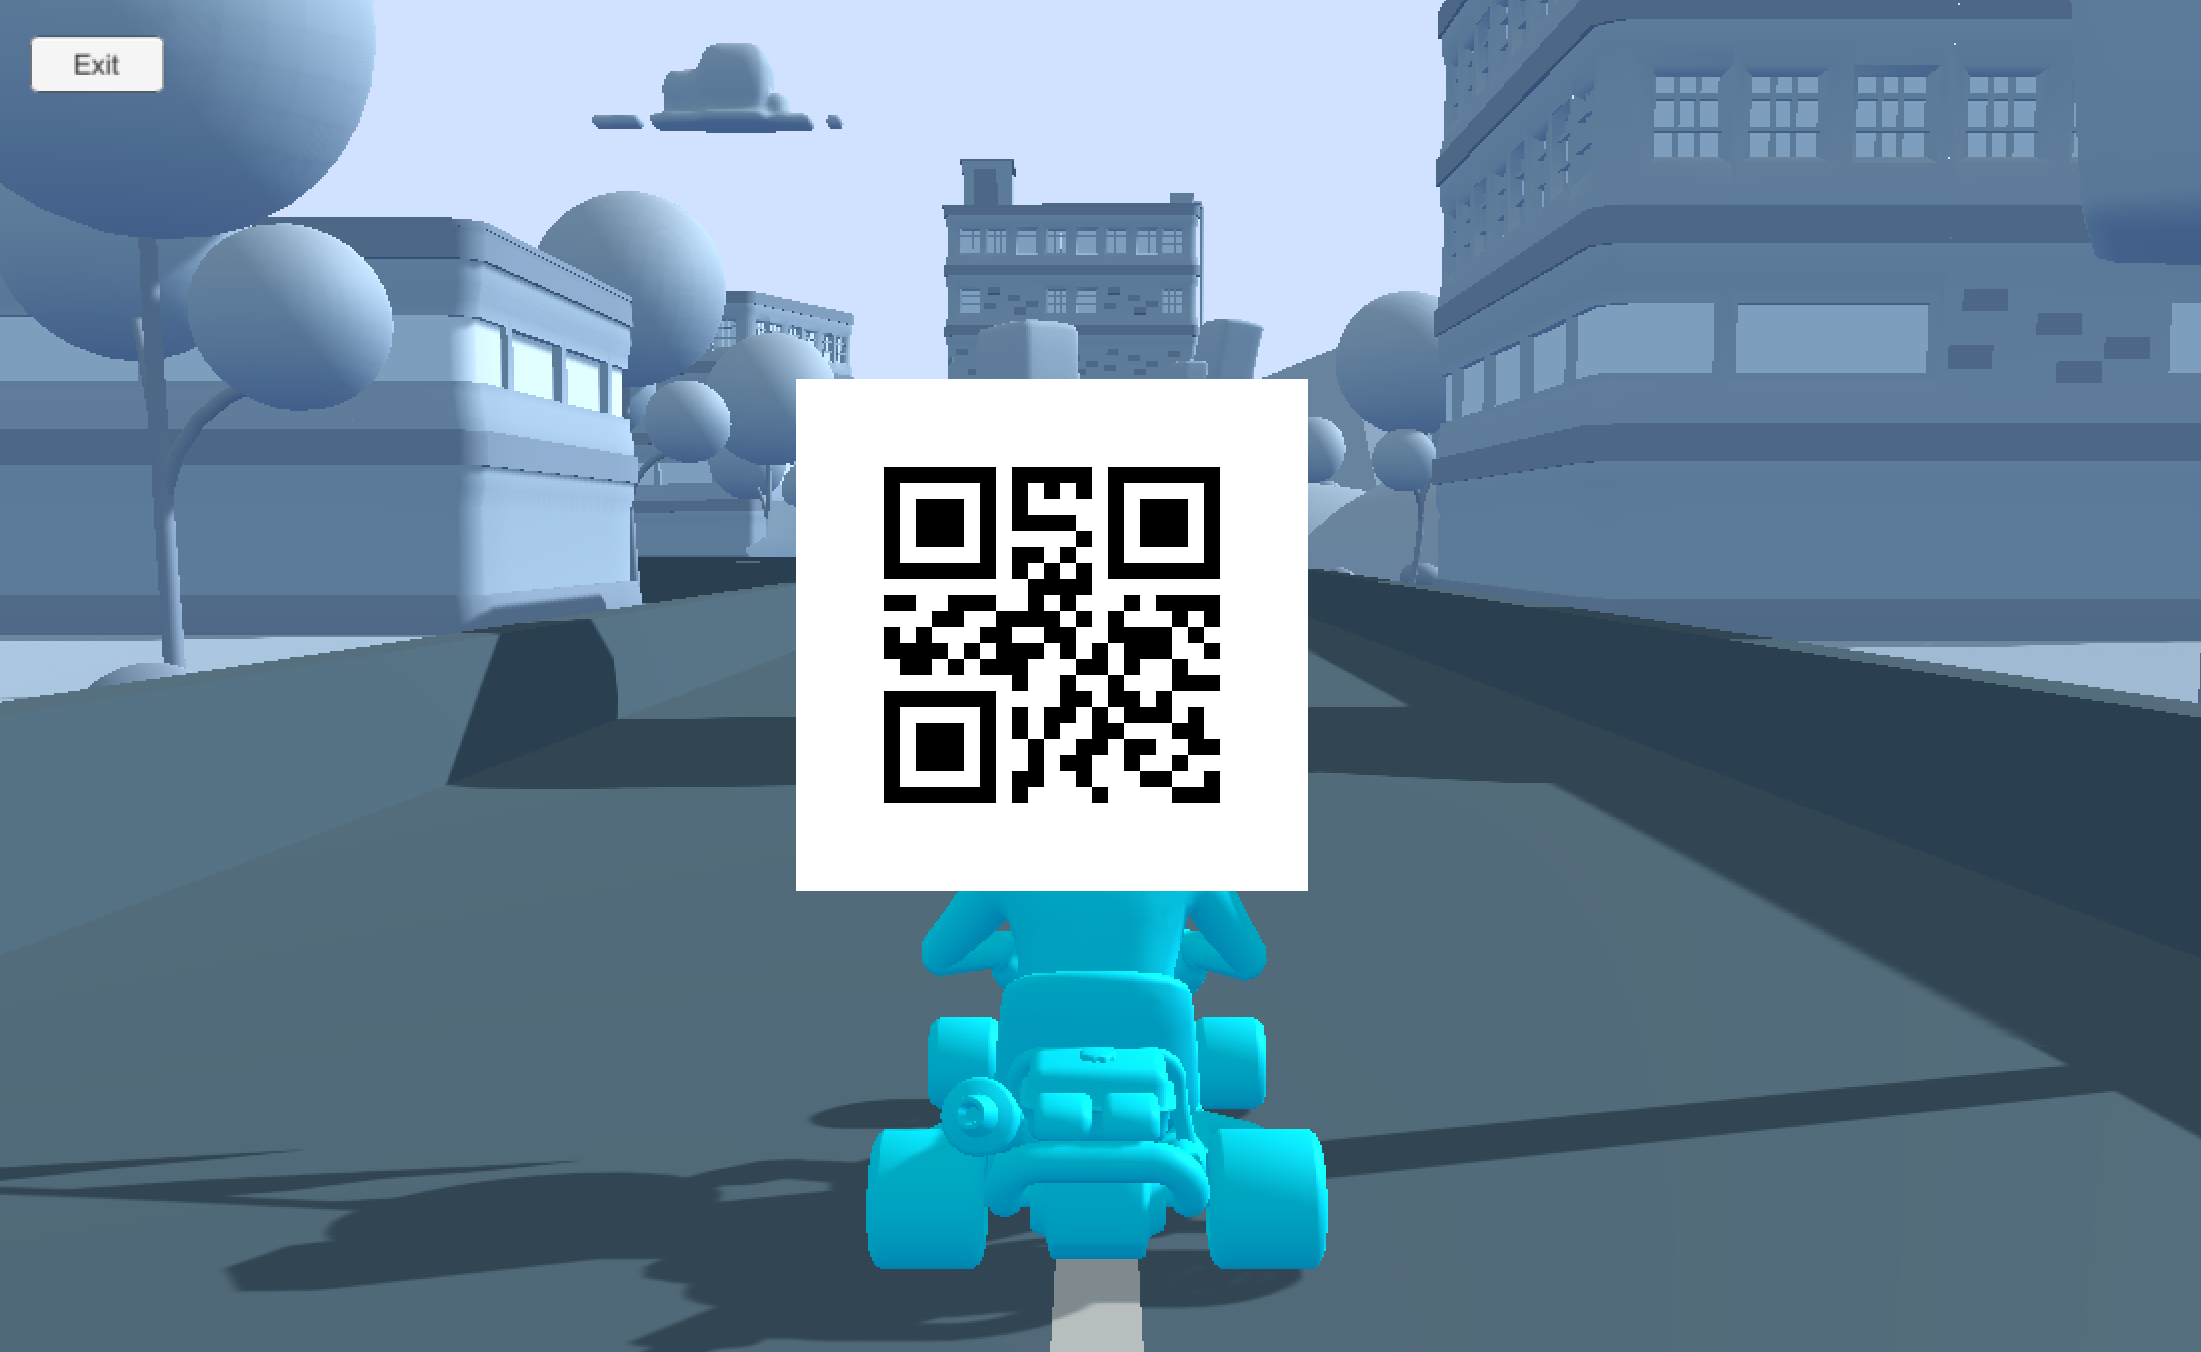
\includegraphics[width=0.90\textwidth]{./Imagenes/Bitmap/pruebaQR.png}
    \caption{Prueba del uso del QR para iniciar juego}
\label{Fig:QR}
\end{figure}



Para la utilizaci\'on de la librer\'ia debe incluirse un \textit{GameObject} en la escena que contenga un componente que la utilice. En la soluci\'on propuesta, este objeto es el encargado de iniciar el servidor y mostrar el QR para que el m\'ovil pueda iniciar la conexi\'on. Adem\'as, esta clase debe dar la opci\'on de a\~nadir un nuevo \textit{listener} de la interfaz \textit{InputMovileInterface} para recibir los mensajes del m\'ovil. La \'ultima funci\'on de este componente es la de preparar las im\'agenes que se van a enviar al dispositivo Android y enviarlas. Este proceso debe hacerse en la funci\'on \textbf{LateUpdate()} ya que esta funci\'on de Unity es llamada por el motor al final de cada ciclo de ejecuci\'on. Esto sirve para asegurarse que la textura que se captura de la c\'amara no va a sufrir alteraciones en ese \textit{frame}. Para conseguir esto, debe incluirse en el proyecto una nueva c\'amara de Unity de la que poder extraer la textura que se va a enviar por red. Una vez se tenga esta textura, se comprimir\'a en formato PNG y se enviar\'a utilizando la librer\'ia.\\

Para que los mensajes que llegan del m\'ovil sean tratados se ha implementado la clase \textbf{MobileInput}. Esta clase es la versi\'on del \textit{input} adaptada al uso de la librer\'ia. En esta clase se tienen guardados cada uno de los botones del mando con sus coordenadas (x,y), ancho y alto. Esto nos permite comparar las coordenadas de las pulsaciones del usuario con la posici\'on virtual de los botones del mando que se han definido previamente. En caso de que la pulsaci\'on se encuentre dentro de las coordenadas del bot\'on, la pulsaci\'on se da como correcta. Como cada m\'ovil usa unas dimensiones diferentes, esta clase es la encargada de escalar la posici\'on de los botones virtuales iniciales una vez el dispositivo m\'ovil manda sus dimensiones. Por \'ultimo, esta clase se encarga de recibir el mensaje de desconexi\'on del m\'ovil. En este ejemplo se ha optado por reiniciar el servidor. \\

En este ejemplo se ha querido mantener la opci\'on de jugar tanto con los controles originales como usando el m\'ovil. Para conseguir esto se ha implementado la clase \textbf{SelectController}, lo que permite al usuario final elegir cu\'al de las 2 opciones de \textit{input} quiere usar para jugar. \\

\begin{figure}[!ht]
     \subfloat[Men\'u Principal Juego\label{}]{%
       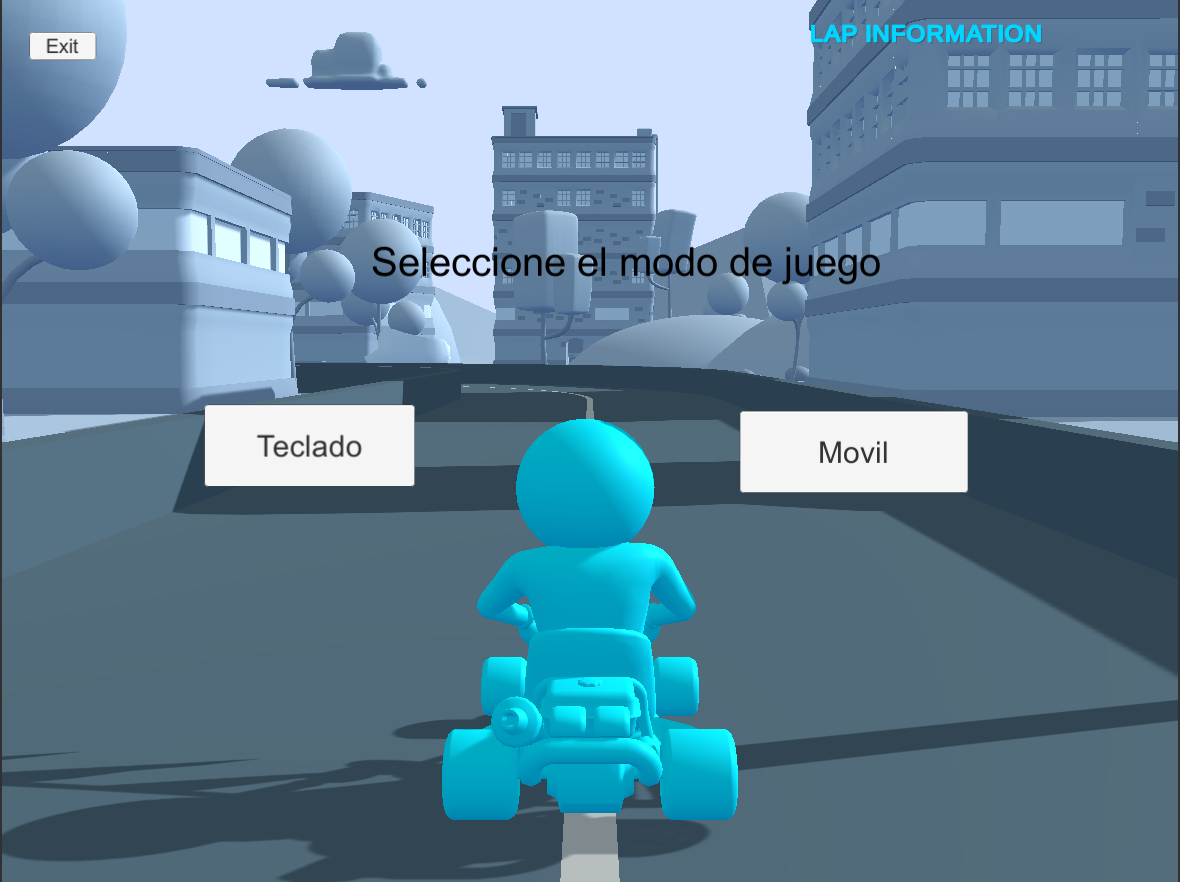
\includegraphics[width=0.5\textwidth]{./Imagenes/Bitmap/Menu_Principal_Juego}
     }
     \hfill
     \subfloat[Ejemplo de mando en Android\label{}]{%
       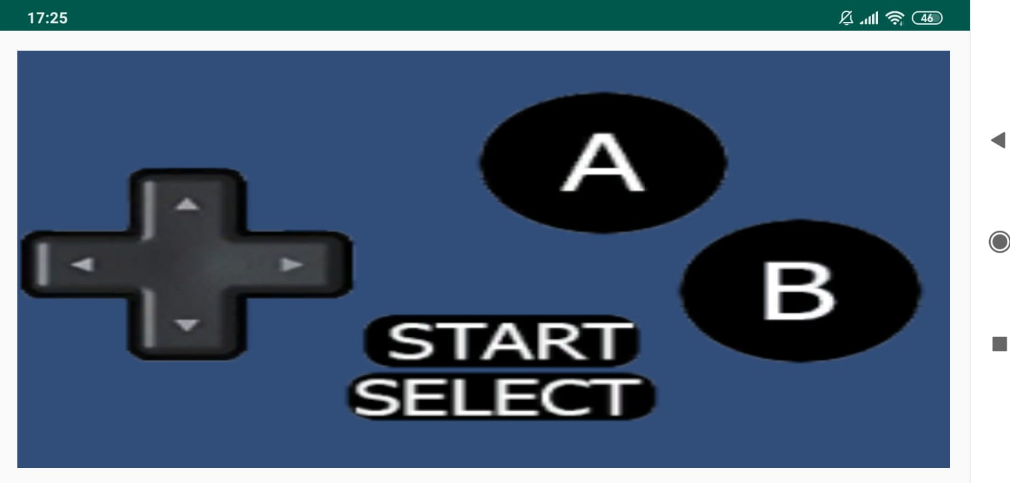
\includegraphics[width=0.5\textwidth]{./Imagenes/Bitmap/Mando}
     }
     \label{fig:quinta}
   \end{figure}


%-------------------------------------------------------------------
\section{Objetivos y organizaci\'on de las pruebas}
%-------------------------------------------------------------------

Previo a las pruebas con usuarios se definieron una serie de objetivos que cubrir durante la evaluaci\'on. Estos objetivos son los siguientes:

\begin {itemize}
\item Comprobaci\'on del funcionamiento de ambas aplicaciones (Android y Unity) en diferentes configuraciones.
\item Rendimiento de la parte de red, sobretodo en el env\'io de im\'agenes y el tiempo de env\'io de las pulsaciones.
\item Valorar c\'omo de intuitivo es el uso de la herramienta.
\end {itemize}

Para comprobar si el rendimiento de los diferentes procesos que realizan las aplicaciones para comunicarse se han implementado rastreadores o \textit{trackers} en las aplicaciones. Estos \textit{trackers} son clases y m\'etodos cuya funci\'on es la de llevar la cuenta del tiempo que tardan cada una de las diferentes acciones que se realizan. Se ha implementado un \textit{tracker} que se encarga de comenzar a contar cuando el usuario realiza una pulsaci\'on y para de contar una vez la aplicaci\'on recibe el mensaje de vibraci\'on. Este proceso es un ciclo completo de interacci\'on de usuario, lo que nos permite comprobar cu\'anto es el retardo que experimenta el usuario al interactuar.\\

Adem\'as de este \textit{tracker}, se han implementado dos m\'as para controlar la compresi\'on y la descompresi\'on del PNG. La compresi\'on del PNG se realiza en Unity y la descompresi\'on se realiza en Android. Estos datos son recolectados en el juego y plasmados en un documento de texto para su posterior tratamiento. Estos datos nos ayudar\'an a saber cu\'anto tarda el frame desde que es recogido por la c\'amara en Unity hasta que es descomprimido y plasmado al usuario en el m\'ovil. \\

El rendimiento de ambas aplicaciones es dependiente del \textit{hardware} del m\'ovil y del ordenador ya que se utilizan varios hilos de ejecuci\'on de manera simult\'anea y el trabajo de compresi\'on y descompresi\'on del PNG requiere de un tiempo que puede incrementar si el procesador trabaja a frecuencias demasiado bajas. Es por esto que los \'ultimos datos que el \textit{tracker} extrae del usuario son el modelo de procesador, tarjeta gr\'afica y memoria RAM del ordenador. Para los datos del dispositivo m\'ovil se le pide al usuario que lo indique en un formulario posterior a la prueba.\\

Se ha dise\~nado un proceso de pruebas que maximice la libertad de los usuarios a la hora de jugar. Lo que se ha decidido controlar son las diferentes etapas del test. El proceso de la prueba es igual para todos los usuarios. Al extraer los datos mientras el usuario juega, no importa c\'omo juegue el usuario ni que pruebe una mec\'anica en espec\'ifico. El \'unico requisito es que la conexi\'on se cierre de manera por lo menos una vez por usuario ya que es en este momento cuando el m\'ovil env\'ia los datos recogidos por el \textit{tracker} al ordenador para realizar el documento de texto con los datos almacenados. La decisi\'on de realizar el env\'io de los datos al final es para enviar sobrecargar la red con m\'as env\'ios de datos, de esta manera tanto la latencia de red como la carga de los dispositivos no se ve afectada por el \textit{tracker}. Las pautas para la realizaci\'on de las pruebas han sido las siguientes:\\

\begin {itemize}
\item Se informa al usuario de los datos t\'ecnicos que se van a extraer de esta prueba (modelo de tarjeta gr\'afica, modelo de procesador, memoria RAM) y del posterior formulario a rellenar.
\item Se ha subido el ejecutable y el APK a un repositorio p\'ublico para que el usuario pueda hacer las pruebas.
\item Se ha indicado al usuario que el ordenador y el m\'ovil deben estar conectados a la misma red WIFI.
\item Se ha utilizado la aplicaci\'on de \textbf{Discord} para realizar una llamada con el usuario y que este compartiese la pantalla donde se estaba ejecutando el juego.
\item Se ha explicado al jugador que tiene que escanear el c\'odigo QR que aparece en el juego con la aplicaci\'on que se ha descargado del repositorio.
\item Se ha indicado al usuario que debe dar varias vueltas al circuito para que los datos puedan recogerse. 
\item Se ha realizado una entrevista con el usuario de entre 5 y 10 minutos para rellenar el formulario y comentar cualquier tipo de \textit{feedback} sobre la herramienta y el juego.
\end {itemize}

Al final de la prueba se realiza una charla con el usuario donde este nos indica todas las observaciones, sugerencias de mejora y puntos positivos. En esta charla tambi\'en se hacen las siguientes preguntas:

\begin {itemize}
\item Indique modelo de m\'ovil que ha usado para la prueba.
\item Describa su trasfondo en el mundo de videojuegos. (Juegos normalmente jugados por usted y en que dispositivos, etc)
\item Valore del 1 al 8 la fluidez a la hora de jugar (Siendo 1 - Mala y 8 - Excelente)
\item Describa si fuese necesario alg\'un cambio en lo referente a la vibraci\'on del dispositivo al pulsar.
\end {itemize}

%-------------------------------------------------------------------
\section{Resultados de las pruebas}
%-------------------------------------------------------------------

%-------------------------------------------------------------------
\subsection{Pruebas de rendimiento}
%-------------------------------------------------------------------

Para comprobar la eficiencia de la librer\'ia desarrollada, se ha procedido a realizar una serie de pruebas con usuarios en las que se han hecho mediciones del tiempo que tardan los procesos principales. Los procesos que se han medido son tanto la compresi\'on de las im\'agenes que se realizan en Unity para ser enviadas por red como la descompresi\'on de estas mismas im\'agenes una vez llegan al m\'ovil.\\

El procedimiento que se ha seguido para hacer estas mediciones ha sido el de jugar durante 5 minutos al juego. La preparaci\'on y proceso de las pruebas est\'an detalladas en la secci\'on anterior. Los usuarios han probado la herramienta en sus hogares y utilizando los siguientes dispositivos:

\begin{table}[h]
    \begin{tabular}{ccccc}
        \toprule
         \textbf{Usuarios} & \textbf{M\'ovil} & \textbf{Procesador} & \textbf{RAM} & \textbf{Gr\'afica} \\
        \midrule
\textbf{Usuario 1} & One Plus 6 & i7-5820K 3.30GHz & 32GB &  GTX 980\\
\textbf{Usuario 2} & One Plus 6 & i7-3630QM 2.4GHz & 6GB &  Intel 4000 \\
\textbf{Usuario 3} & S9+ & Intel Q9400 2.66GHz & 8GB &  GTX 740 \\
\textbf{Usuario 4} & S8 & i7-6700HQ 2.6GHz & 16GB & GTX 960M \\
\textbf{Usuario 5} & S9+ & i7-5820K 3.3GHz & 32GB &  GTX 980 \\
        \bottomrule
    \end{tabular}
\caption{Sistemas utilizados por cada usuario durante las pruebas}
\label{tablausuarios}
\end{table}

Los tiempos se han medido en milisegundos (ms) y para que el volumen de datos sea semejante en todos los usuarios, el tiempo de ejecuci\'on ha sido de 5 minutos para todas las pruebas. Los datos de las pruebas han sido los siguientes:

\begin{figure}[h]
     \subfloat[Descompresi\'on de PNG en Android\label{}]{%
       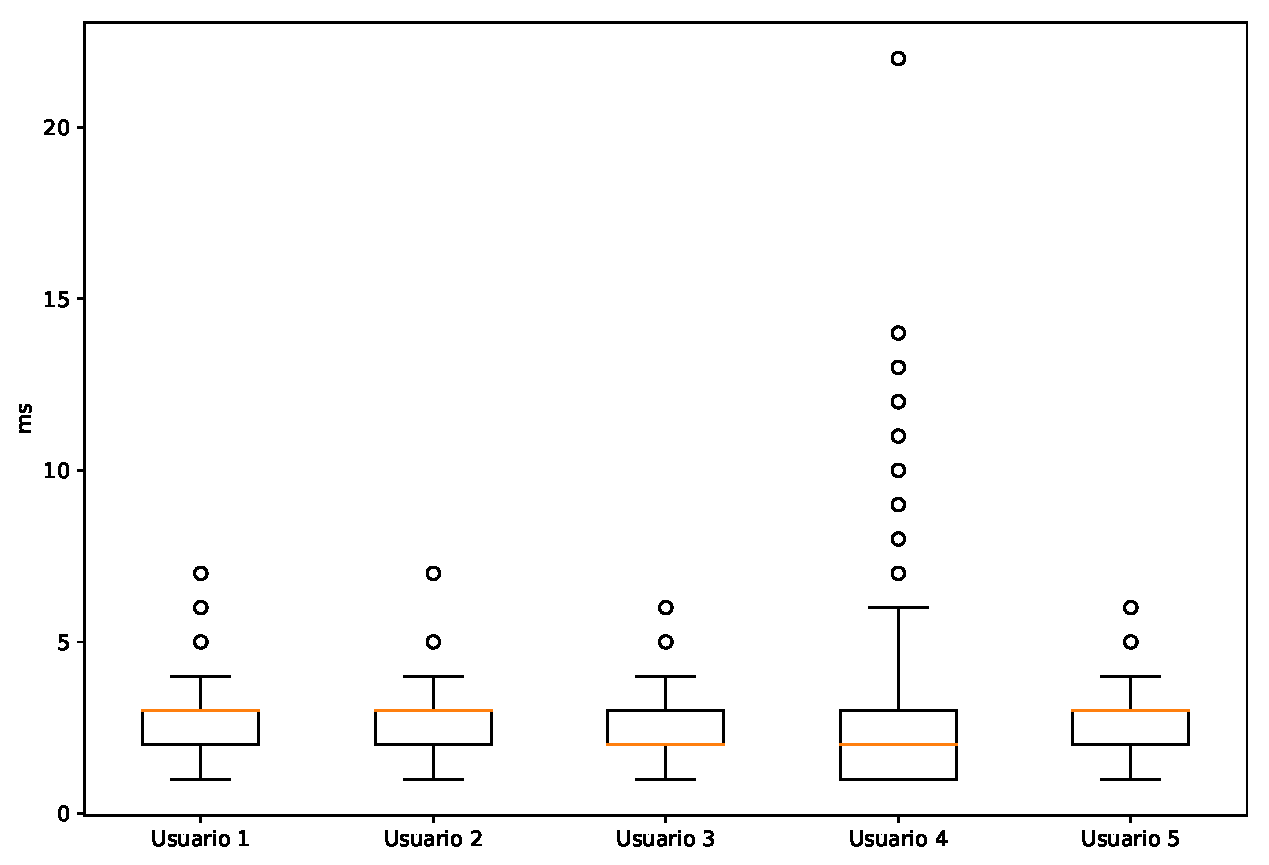
\includegraphics[width=0.5\textwidth]{./Imagenes/Vectorial/AndroidCompresion.pdf}
     }
     \hfill
     \subfloat[Compresi\'on de PNG en Unity\label{}]{%
       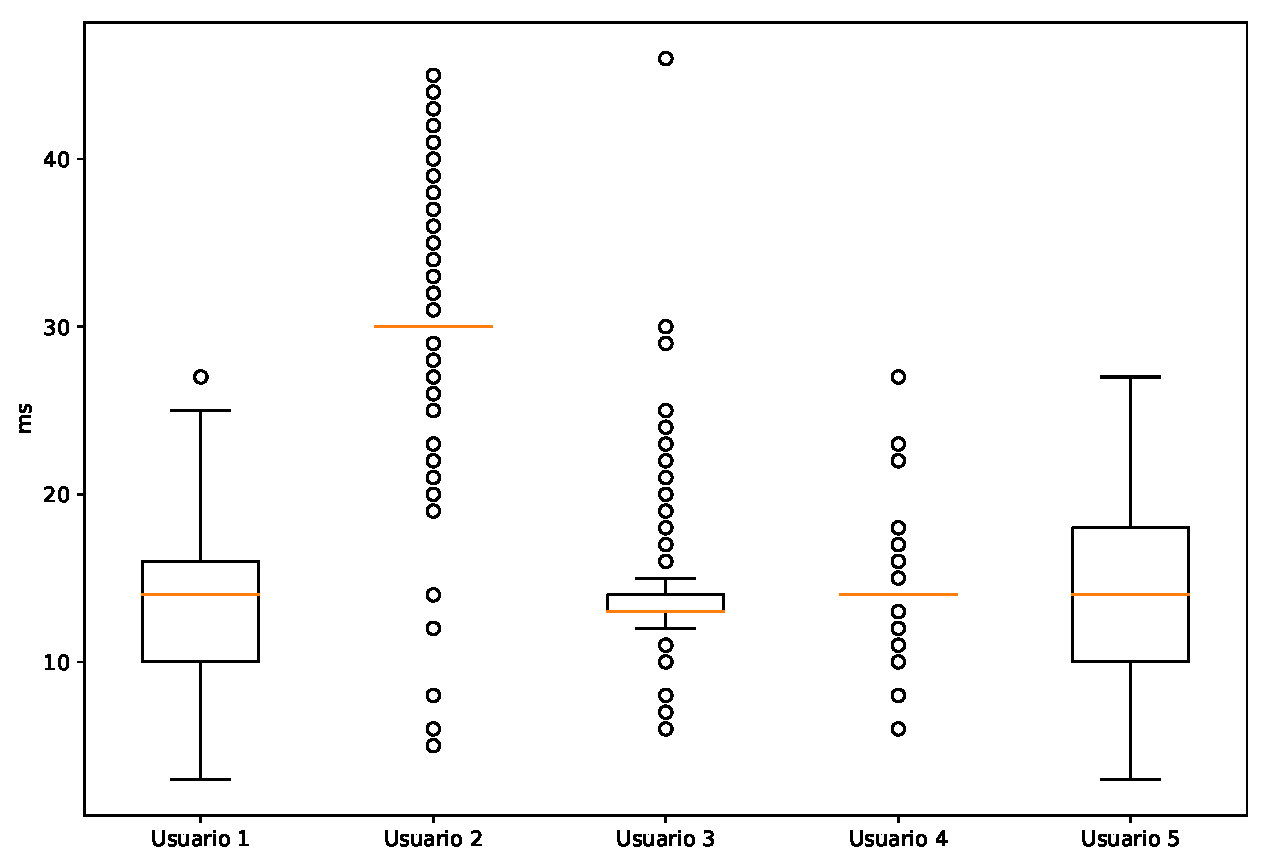
\includegraphics[width=0.5\textwidth]{./Imagenes/Vectorial/UnityCompresion.pdf}
     }
	\caption{Tiempo de compresi\'on y descompresi\'on de las im\'agenes}
     \label{}
   \end{figure}



Los datos obtenidos de las pruebas muestran que la descompresi\'on de las im\'agenes en Android mantiene unos tiempos uniformes. Se ha calculado la desviaci\'on est\'andar total y se ha obtenido 0.8756. Esto indica que los datos se encuentran cercanos al valor de la media excepto en el Usuario~4. La desviaci\'on est\'andar de este usuario es de 1.2183, lo que indica una mayor inestabilidad a la hora de descomprimir las im\'agenes. Esto durante una sesi\'on de juego crea inestabilidades en la tasa de refresco de im\'agenes. \\

Los datos extra\'idos de la compresi\'on de im\'agenes en Unity muestran que una desviaci\'on est\'andar bastante superior a los valores de Android. La desviaci\'on est\'andar total es de 2.3729, lo que indica una alta dispersi\'on respecto de la media. Esto se debe a que tanto el usuario 1 como el 5 cuyas desviaciones est\'andar son 3.7834 y 4.6872 respectivamente disparan la ponderaci\'on media de la desviaci\'on est\'andar total. A pesar de esta desviaci\'on, los m\'aximos y m\'inimos est\'an por debajo de los 27 milisegundos.  Estos datos se traducen en que se pueden llegar a comprimir 70 fotogramas en un segundo en el mejor de los casos.\\



De media, los dispositivos Android utilizados en las pruebas muestran un valor de 2.6 milisegundos a la hora de descomprimir las im\'agenes recibidas. Los dispositivos utilizados para jugar muestran un tiempo medio de compresi\'on de im\'agenes de 17 milisegundos. Esto se traduce en un tiempo medio conjunto de 19.6 milisegundo. A esto, se tiene que sumar que durante la ejecuci\'on de las pruebas hab\'ia una latencia de red de 2 milisegundos. Esto nos deja con un total de 21.6 milisegundos como tiempo total desde que el fotograma es comprimido hasta que este se descomprime y muestra en el m\'ovil. Traducido a fotogramas por segundo esto tendr\'ia un valor de aproximadamente 46.

%-------------------------------------------------------------------
\subsection{Resultados del test de opini\'on posterior a las pruebas}
%-------------------------------------------------------------------

Una vez se ha terminado la prueba de la librer\'ia, se somete al usuario a una charla de 5 minutos donde este puede comentar cualquier aspecto a mejorar del juego. Durante esta charla se ha realizado un cuestionario. Los resultados de los cuestionarios arrojan resultados similares a los vistos en las gr\'aficas. La experiencia durante la sesi\'on fue satisfactoria para todos los usuarios pero fue el usuario~2 el que dio una respuesta m\'as negativa. Esto es debido a tirones y bajadas de fotogramas que sufridas durante la prueba. A pesar de esto, el usuario indic\'o que pudo jugar sin complicaciones la mayor parte del tiempo.

\begin{table}[h]
\adjustbox{max width=\textwidth}{
    \begin{tabular}{ccc}
        \toprule
         \textbf{Usuarios} & \textbf{Valoraci\'on de la fluidez} & \textbf{Valoraci\'on del efecto de vibraci\'on} \\
        \midrule
\textbf{Usuario 1} & 8 & Adecuada.\\
\textbf{Usuario 2} & 5 & Normal. \\
\textbf{Usuario 3} & 7 & Buena.\\
\textbf{Usuario 4} & 7 & Adecuada. \\
\textbf{Usuario 5} & 8 & Preferiblemente mantener vibraci\'on al mantener el bot\'on. \\
        \bottomrule
    \end{tabular}}
\caption{Resultados del test realizado a los usuarios posterior a la prueba}
\label{opinionesusuarios}
\end{table}


%-------------------------------------------------------------------
\section{An\'alisis y discusi\'on de los resultados}
%-------------------------------------------------------------------
La ejecuci\'on de las pruebas demuestra que las ejecuciones en Android son estables en aquellos dispositivos en los que se ha probado. Unity por su parte, aunque consiga los requisitos m\'inimos en gamas bajas llegando a las 30 compresiones por segundo y en gamas superiores llegando a las 70, sigue entrando  dentro de los l\'imites aceptados por la industria de entre 30 y 60 fotogramas por segundo. Por desgracia, la tasa de compresi\'on al tener una desviaci\'on est\'andar alta hace a esta velocidad de compresi\'on demasiado inestable. Esto provoca que puedan apreciarse en el dispositivo m\'ovil cambios bruscos en la tasa de refresco, lo que puede llegar a crear molestias en el usuario a la hora de jugar. Esto tambi\'en impide el uso de la pantalla de m\'ovil como pantalla principal, lo que obliga estrictamente a usar la pantalla del m\'ovil como pantalla secundaria.\\

Tambi\'en podemos observar que los datos del Usuario~2 muestran que la ejecuci\'on de este usuario no ha sido satisfactoria debido al tiempo que tarda Unity en comprimir las im\'agenes. De media, este usuario es capaz de comprimir 30 fotogramas por segundo. Este dato entra dentro de las medidas est\'andar de la industria pero est\'a demasiado ajustado ya que los fotogramas m\'inimos aceptados en la industria son 30.\\

Al optar por un modelo de librer\'ia vers\'atil para el desarrollador, la optimizaci\'on de la compresi\'on de im\'agenes recae sobre \'el de manera directa tanto positiva como negativamente. Es decir, la velocidad de compresi\'on y su estabilidad dependen de los algoritmos de compresi\'on a usar y del momento en el que se ejecuten.\\



% Variable local para emacs, para  que encuentre el fichero maestro de
% compilaci�n y funcionen mejor algunas teclas r�pidas de AucTeX
%%%
%%% Local Variables:
%%% mode: latex
%%% TeX-master: "../ManualTeXiS.tex"
%%% End:
